\documentclass[14pt]{beamer}
\usetheme{default}
\setbeamertemplate{navigation symbols}{}
\usepackage{graphics}
\usepackage{array}
\usepackage{verbatim}
\usepackage{hyperref}

\title{Paxos on (a) many-core platform(s)}
\author{Motiejus Jak\v{s}tys \\
1003704j}

\date{March 2013}

\begin{document}

\begin{frame}[plain]
    \titlepage
\end{frame}

\begin{frame}
    \frametitle{Table of Contents}
    \tableofcontents
    Interrupt any time.
\end{frame}

\section{Changes in many-core platforms}

\begin{frame}{Laws}
    \begin{tabular}{cm{0cm}}
            Pollack's rule &
            \pause
            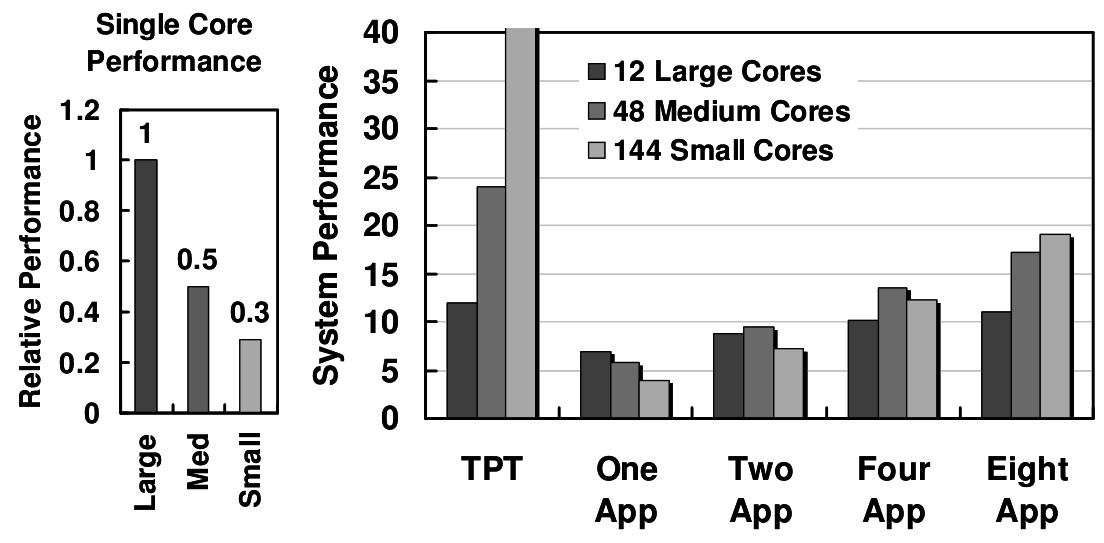
\includegraphics[height=0.4\textheight]{images/pollack.png}
            \\
            Amdahl's law &
            \pause
            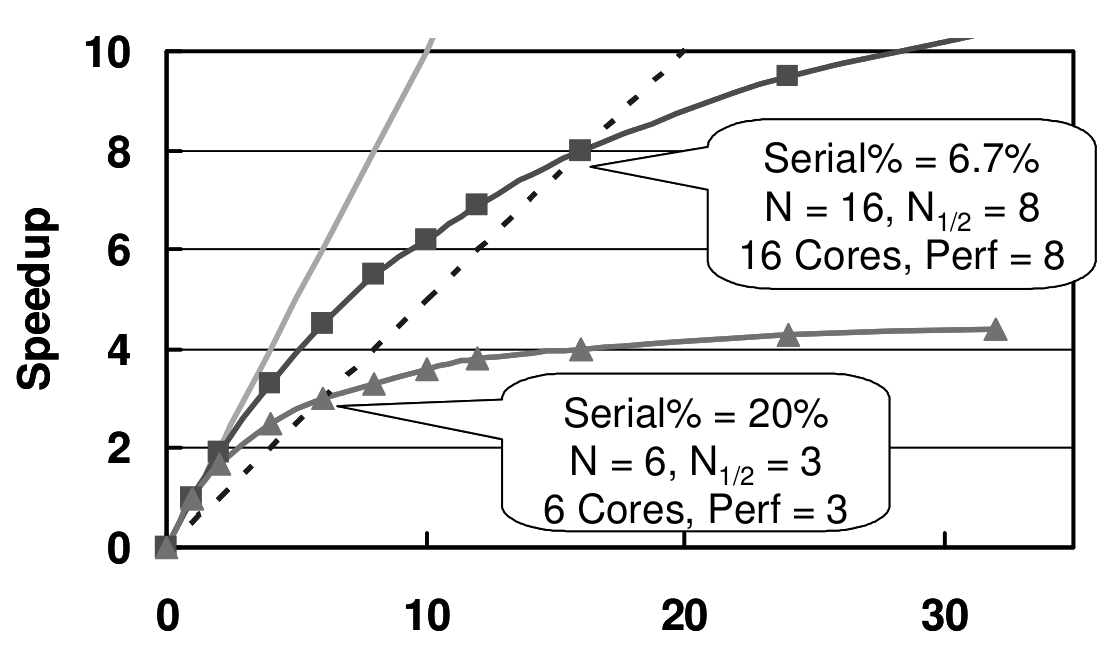
\includegraphics[height=0.4\textheight]{images/amdahl.png} \\
    \end{tabular}
\end{frame}

\begin{frame}{So?}
    \begin{itemize}
        \item Increase number of cores.
        \item And make them smaller.
            \pause
        \item \alert{Increase parallelism}
    \end{itemize}
    
\includegraphics[height=0.2\textheight]{images/orly.jpg}
\end{frame}

\section{Trends}

\begin{frame}{Tilera}
    \pause
    \begin{center}
        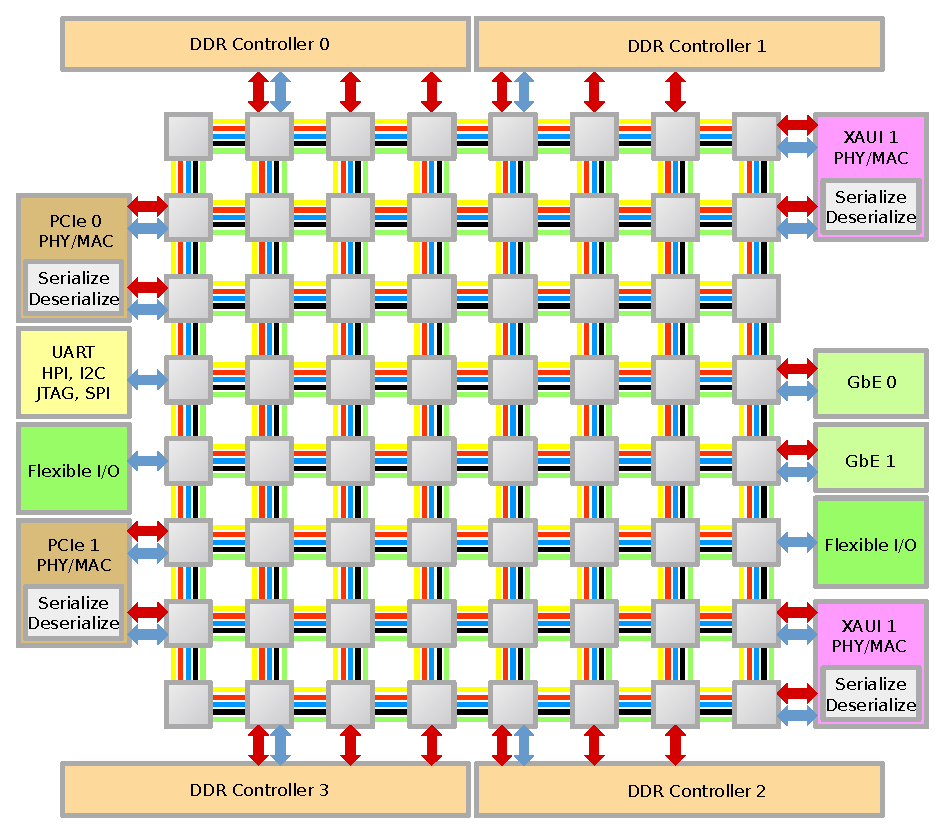
\includegraphics[height=0.8\textheight]{images/tile64.pdf}
    \end{center}
\end{frame}

\begin{frame}{Cluster?}
    \begin{center}
        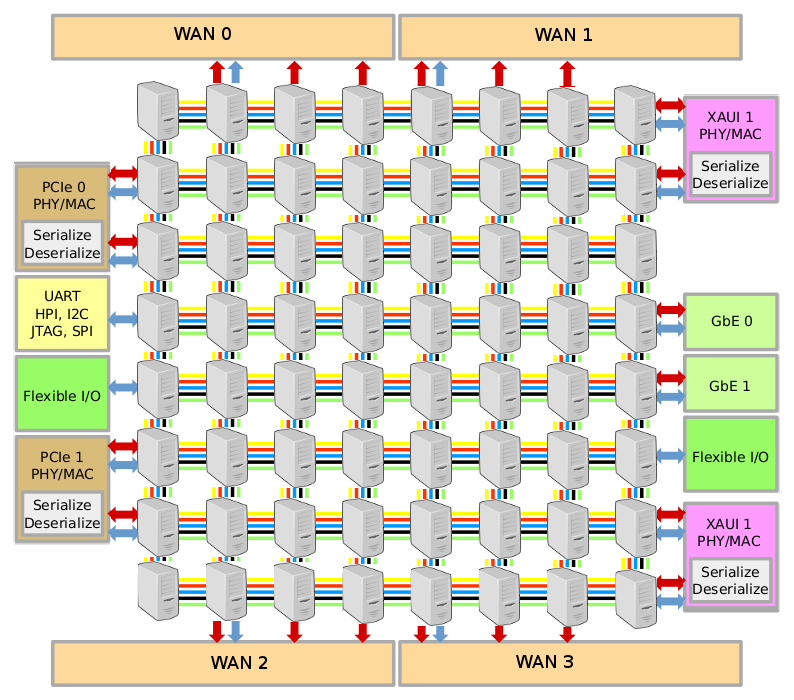
\includegraphics[height=0.8\textheight]{images/computer_clusterb.png}
    \end{center}
\end{frame}

\begin{frame}{More trendy hardware}
    \begin{center}
        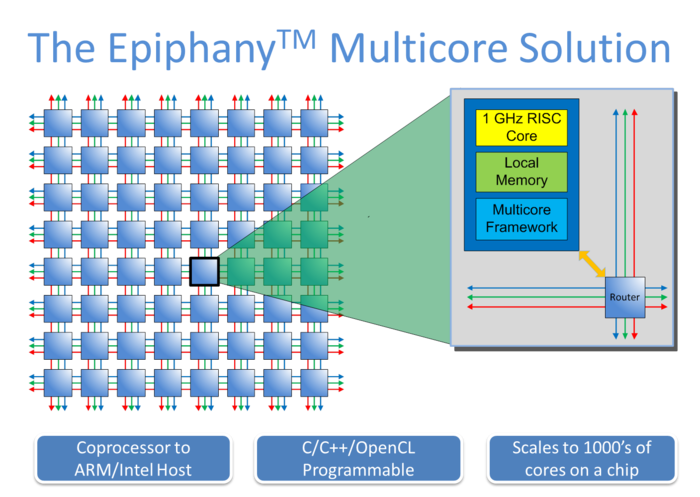
\includegraphics[height=0.8\textheight]{images/parallella_64core.png}
    \end{center}
\end{frame}

\begin{frame}{Even less chips}
    \begin{center}
        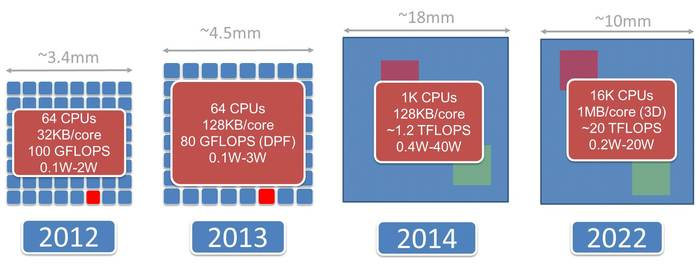
\includegraphics[width=\textheight]{images/parallella_future.jpg}
    \end{center}
\end{frame}

\begin{frame}{Recap}
    \begin{itemize}
        \item Reduce serial component
        \item Parallelization is complex to program (elaborate!)
            \pause
        \item Need redundancy to be robust
    \end{itemize}
\end{frame}

\section{Paxos}

\begin{frame}{Paxos}
    \pause
    \vspace{0.35cm}
    \hskip0.6cm
    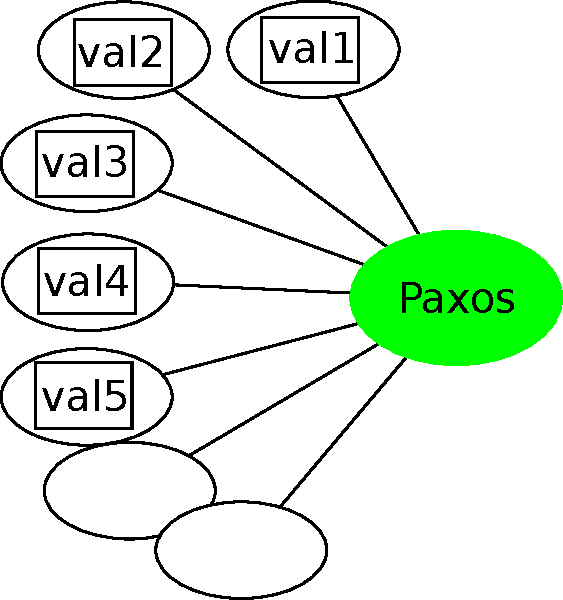
\includegraphics[height=5cm]{images/paxos1.pdf}
\end{frame}

\begin{frame}{Paxos}
    \vspace{0.35cm}
    \hskip0.6cm
    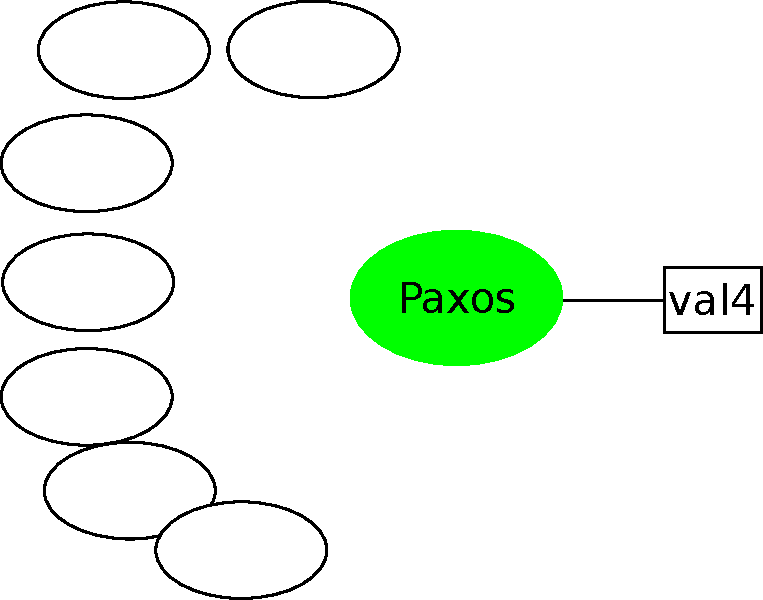
\includegraphics[height=5cm]{images/paxos2.pdf}
\end{frame}

\begin{frame}{Paxos}
    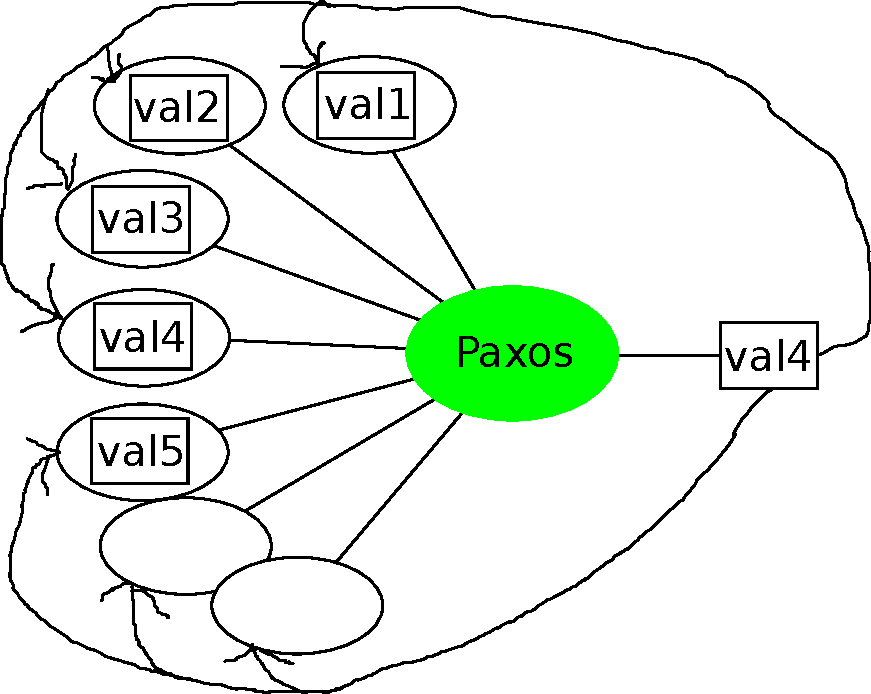
\includegraphics[height=5.87cm]{images/paxos3.pdf}
\end{frame}

\section{Language choice}

\begin{frame}{Language choice}
    \pause
    
\includegraphics[width=\textwidth]{images/cloudhaskell.png}
    \pause
    \vspace{1cm}

    But ... (demonstration)
\end{frame}

\begin{frame}{Erlang}
    \begin{columns}
        \column{.8\textwidth}
        \begin{itemize}
            \item<1> Provides what Cloud Haskell tried to!
            \item<1> Message passing
            \item<1> Concurrent, distributed
            \item Loosely typed
        \end{itemize}
        \column{.19\textwidth}
        
\includegraphics[width=\textwidth]{images/erlang-logo.pdf}
    \end{columns}
    \pause
    \vspace{2cm}
    Changed algorithm implementation.
\end{frame}

\section{Benchmarks}

\begin{frame}{Bad embarrassingly parallel Benchmarks}
    \pause
        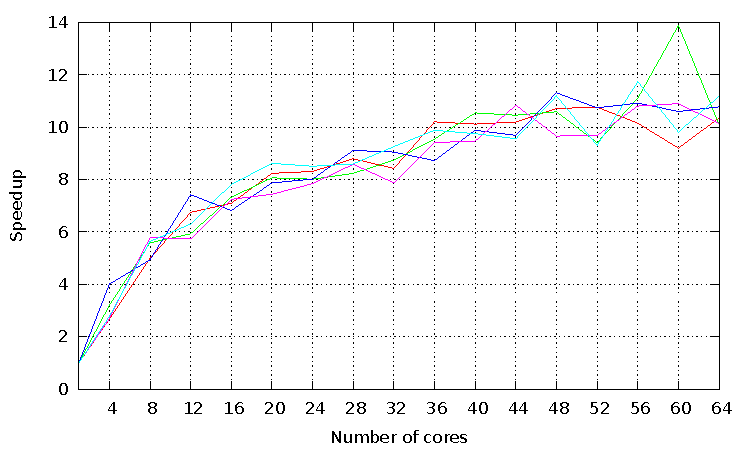
\includegraphics[width=\textwidth]{images/bad_speedup.pdf}
\end{frame}

\begin{frame}{Good embarrassingly parallel Benchmarks}
    \includegraphics[width=\textwidth]{images/speedup.pdf}
\end{frame}

\begin{frame}{Good embarrassingly parallel Benchmarks}
    \includegraphics[width=\textwidth]{images/slowdown.pdf}
\end{frame}

\begin{frame}[fragile]{Implemented Classic Paxos\footnote{
    \url{https://github.com/Motiejus/epaxos}}}

        \fontsize{11pt}{14}\selectfont \begin{verbatim}
-type fsmref() :: reference().
-type value() :: term().
-type learner_callback() :: fun((value()) -> ok).

%% Specify learner function per election.
%% Function will be executed when a value is learned.
-spec init_learner(fsmref(), learner_callback()) -> ok.

%% Executed by application.
-spec propose(fsmref(), value()) -> ok.
    \end{verbatim}
\end{frame}

\section{Summary \& future work}

\begin{frame}{Year 4}
    \begin{tabular}{|l|l|}
        \hline
        TILEPro64 dev env & 2 weeks \\ \hline
    Haskell investigation & 4 weeks \\ \hline
  Port Erlang to TileMDE3 & 1 hour \\ \hline
              Make it run & 3 weeks \\ \hline
   Try to understand FGGC & 4 weeks \\ \hline
          Implement Paxos & 1 week \\ \hline
                   Report & 2 weeks \\ \hline \hline
               \bf{TOTAL} & \bf{16 weeks} \\ \hline
    \end{tabular}
\end{frame}

\begin{frame}{Future work}
    \pause
    Erlang message passing via UDN
    \pause

    \vskip.7cm
    Paxos at work!

    \begin{center}
        
\includegraphics[height=.5\textheight]{images/spilgames.png}
    \end{center}
\end{frame}

\end{document}
